\documentclass[12pt, letterpaper]{report}
\usepackage{graphicx}
\usepackage{hyperref}
\usepackage{amssymb}
\usepackage{amsmath}
\usepackage{float}
\usepackage{mathtools}
\usepackage{enumitem}
\usepackage[margin=1in]{geometry}
\usepackage[figurename=Figura]{caption}
\title{Actividad: Esferas con misma carga y masa}
\author{Juan Pablo Guerrero Escudero, A01706810}
\date{17 abril, 2024}
\begin{document}
\maketitle
\subsection*{Introducción}
En ésta actividad, se analiza la situación en donde dos cargas con la misma masa y carga, están suspendidas en el mismo punto por medio de un hilo o cuerda. Éstas cuerdas 
se repelen debido a que tienen la misma carga, por lo que forman un ángulo $\alpha$ con la vertical. Por lo tanto, en éste reporte 
se realizará un simulador de éste fenómeno en Matlab.  
\subsection*{Código fuente}
\begin{verbatim}
    %% Código Actividad Esferas con misma carga 

    % El usuario ingresa valores de Q, masa y longitud de la cuerda
    Q = input('Ingresa la magnitud de las cargas en Coulombs: '); 
    m = input('Ingresa la masa de las cargas en kg: '); 
    L = input('Ingresa la distancia de la cuerda: '); 
    %Se definen las constantes epsilon cero y aceleración por gravedad 
    e_0 = 8.854e-12; 
    g = 9.81;
    %Se calcula el valor aproximado de beta, para su uso en fzero. 
    beta_aprox = nthroot((Q^2/(16*pi*e_0*L^2*m*g)), 3); 
    %Se crea la función anónima func, la cuál se resolverá numéricamente para 
    func = @(beta) 16.*pi.*e_0.*(L.^2).*m.*g.*((sin(beta)).^2).*(tan(beta))-(Q.^2);     
    
    %Encontrar la raiz con fzero de func, usando valor aproximado beta_aprox,
    %con una tolerancia de 10^-6. 
    root = fzero(func, beta_aprox); 
    %Mostrar el valor resultante con la función disp. 
    disp(['El valor de beta que resuelve la ecuación es: ', num2str(root)]);
    
    %Creación de la gráfica 
    beta_range = linspace(beta_aprox - 5, beta_aprox + 5, 100);  
    func_values = func(beta_range);
    plot(beta_range, func_values, 'b-', 'DisplayName', 'func(beta)');
    xlabel('Beta(radianes)');
    ylabel('func(beta)X');
    title('Gráfico de beta vs func(beta)');
    hold on;
    plot(root, func(root), 'or', 'DisplayName', 'Root');
\end{verbatim}
\subsection*{Explicación}
El código en primer lugar le pide al usuario ingresar los valores de la masa, la carga y la longitud de la cuerda a la que las cargas están unidas. 
Después, se definen las constantes $\epsilon_0$ y $g$, por la aceleración de la gravedad. Después, si observamos el siguiente diagrama: 
\begin{figure}[H]
    \centering
    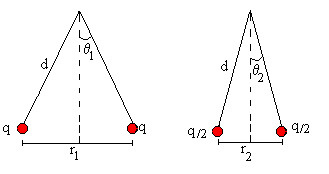
\includegraphics[height = 5cm]{2024-04-17_DiagramaSistemaMismaCarga.jpg}
    \caption{Ángulo de equilibrio en Sistema Electrostático}
\end{figure}
Observamos que, al existir simetría, podemos expresar la $F_e$ como $mg\tan{\alpha}$, y si ésta la igualamos a su fórmula de acuerdo a Coulomb, que dice $F_e = \frac{kQ^2}{r^2}$, obtenemos la expresión 
$mg\tan{\alpha} = \frac{Q^2}{4\pi\epsilon_0r^2}$. Y por lo tanto, $Q^2 = 16\pi\epsilon_0L^2mg\sin{\alpha}^2\tan{\alpha}$. Si buscamos obtener el ángulo de separación dada la masa, la carga de las cargas, y 
la longitud de la cuerda $L$, es imposible analíticamente ya que $\alpha$ se encuentra tanto en la función seno como en tangente. La solución entonces es hacerlo de manera numérica, tratar de encontrar 
la raíz de la función $Q^2$ al igualarla a cero. Para eso, se usa la función $fzero$ que, dada una función anónima y un punto inicial, la función encuentra la raíz de la ecuación. \\ 

Tomando en cuenta que para valores muy pequeños, $\sin{\alpha}\approx \alpha$ y $\tan{\alpha}\approx \alpha$, nuestro mejor valor educado es $\alpha = (\frac{Q^2}{16\pi\epsilon_0L^2mg})^{\frac{1}{3}}$. Ésta fórmula viene de sustituir las funciones trigonométricas en 
la función de $Q^2$.    

\subsection*{Prueba del código}
\begin{enumerate}
\item En la primera prueba se usan los valores $Q = 2x10^{-7} C$, $m = 0.01kg$, y $L = 1.5m$. A continuación los resultados: 
\begin{figure}[H]
    \centering
    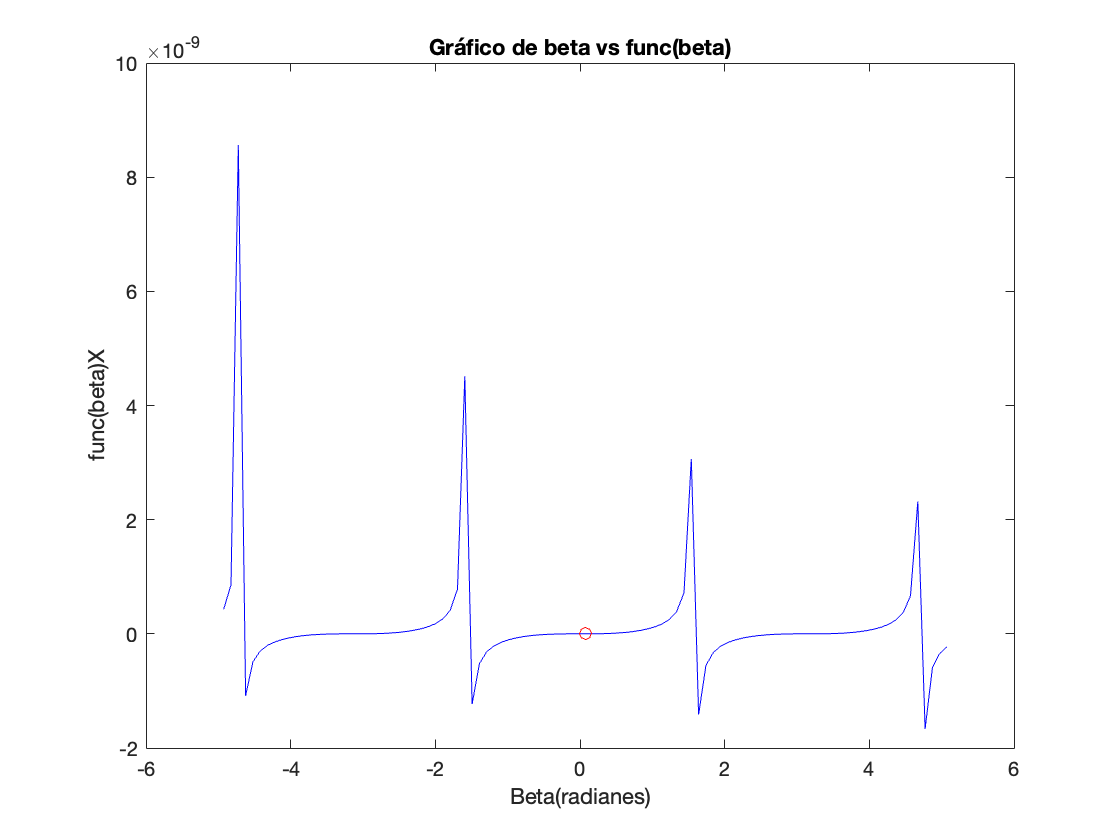
\includegraphics[height = 6cm]{2024-04-17_Grafica1.png}
    \caption{Gráfica de primer caso de prueba}
\end{figure}
Además, resulta que el ángulo de separación calculado es de $\alpha = 0.07412$ radianes. Ésto si se convierte a grados es igual aproximadamente a $4.2468\deg$. Éstos resultados 
son congruentes ya que el ángulo es muy pequeño debido a la escala del sistema, además de que el ángulo es positivo, indicando que las cargas se repelen. Además, la gráfica nos muestra que 
la fuerza eléctrica, en el eje $y$ aumenta y disminuye de forma cíclica, circulando en rojo la raíz encontrada. 
\item El segundo caso de prueba se hace con $Q = 1x10^{-7}C$, $m = 0.01kg$, y $L = 1.5m$. A continuación se muestran los resultados: 
\begin{figure}[H]
    \centering
    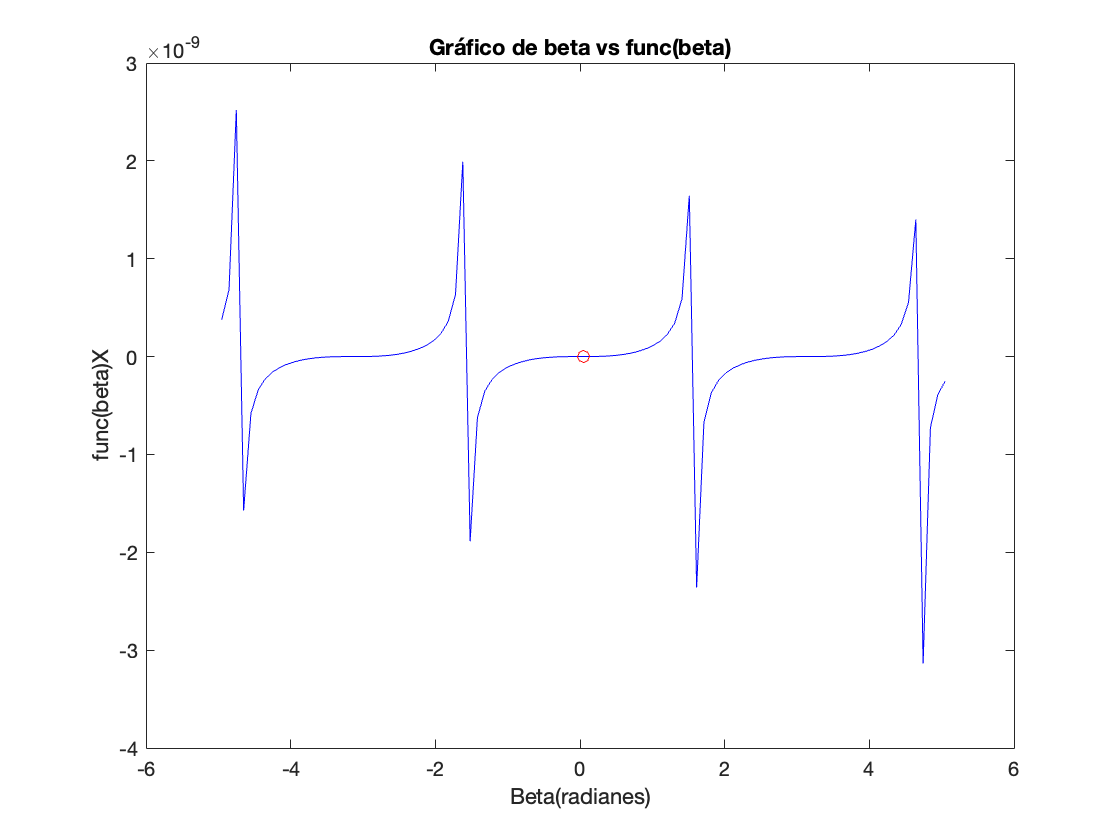
\includegraphics[height = 7cm]{2024-04-17_Grafica2.png} 
    \caption{Gráfica del segundo caso de prueba}
\end{figure}
Además, el ángulo en el cuál éstas fuerzas entran en equilibrio es de $\alpha = 0.046692 $rad, o convertido a grados: $\alpha \approx 2.6753 \deg$. Éstos valores son congruentes ya que 
las cargas son positivas, por lo tanto se repelen. Además, se observa que el ángulo de separación es relativemente pequeño, algo acorde a la escala en la que el sistema está funcionando. 
\end{enumerate}
\subsection*{Conclusión}
En éste trabajo, se realizó una simulación de ángulo de estabilidad entre dos partículas con la misma carga y masa, unidas a una cuerda o hilo con cierta distancia. Se encontró que debido a que en la fórmula 
resultante, no e sposible despejar el ángulo de separación, se usan métodos numéricos para resolverlo, en éste caso, el cruce por cero. En Matlab, ésto es implementado por medio del comando $fzero$, que 
encuentra la raiz o el cruce en 0 del eje y de una ecuación no lineal. Gracias a ésto, el ángulo de separación en radianes es obtenido, y se realizan las gráficas 
correspondientes en cada caso de prueba. \\

Como futuro trabajo, sería una buena dirección tratar de graficar diferentes cantidades dentro de la fórmula, así como buscar posibles sustituciones y ver su relación con 
el campo eléctrico y otros conceptos de la electroestática. 
\end{document}